% Need pgf to compile, may not compile with
%  current stable version, in which case :
%  - download last pgf build from
%    http://media.texample.net/pgf/builds/pgfCVS2009-03-10_TDS.zip
%  - dezip it in /usr/share/local/texmf
%  - run "sudo texhash"

\documentclass[nocover]             % options: RDPonly, coveronly, nocover
{NASA}                       %   plus standard article class options

%\usepackage[utf8]{inputenc}
%\usepackage[T1]{fontenc}
\usepackage{xspace}
\usepackage{graphicx}
\usepackage{times}
%\usepackage[bookmarks=false,colorlinks,linkcolor=blue,urlcolor=blue,citecolor=blue]{hyperref}
\usepackage[bookmarks=false]{hyperref}
\usepackage{varioref}
\usepackage{amsmath}
\usepackage{amssymb}

\renewcommand{\O}[1]{\mathrm{O}\left(#1\right)}
\newcommand{\IGNORE}[1]{}
\newcommand{\N}{\mathbb{N}}
\newcommand{\Z}{\mathbb{Z}}
\newcommand{\C}{\mathbb{C}}
\newcommand{\m}{\mbox}

\newtheorem{mynote}{Note}[section]
  \newcommand{\Note}[1]{\begin{mynote}{\rm {#1}}\end{mynote}}%
\newtheorem{mytheorem}{Theorem}[section]
  \newcommand{\Theorem}[1]{\begin{mytheorem}{\rm {#1}}\end{mytheorem}}%
\newtheorem{mycorollary}{Corollary}[section]
  \newcommand{\Corollary}[1]{\begin{mycorollary}{\rm {#1}}\end{mycorollary}}%
\newtheorem{myremark}{Remark}[section]
  \newcommand{\Remark}[1]{\begin{myremark}{\rm {#1}}\end{myremark}}%
\newtheorem{mylemma}{Lemma}[section]
  \newcommand{\Lemma}[1]{\begin{mylemma}{\rm {#1}}\end{mylemma}}%
\newtheorem{mydefinition}{Definition}[section]
  \newcommand{\Definition}[1]{\begin{mydefinition}{\rm {#1}}\end{mydefinition}}%
\newtheorem{myexample}{Example}[section]
  \newcommand{\Example}[1]{\begin{myexample}{\rm {#1}}\end{myexample}}%
\newtheorem{myalgorithm}{Algorithm}[section]  
  \newcommand{\Algorithm}[1]{\begin{myalgorithm}{\rm {#1}}\end{myalgorithm}}%
\newcommand{\Proof}[1]{\par\noindent{\bf Proof.}~{#1}$\Box$}

\everymath{\displaystyle}
%\setlength{\headheight}{0cm}
%\setlength{\headsep}{0cm}
%\setlength{\topmargin}{0cm}
%\setlength{\oddsidemargin}{0cm} \setlength{\evensidemargin}{0cm}
%\setlength{\textheight}{24cm}
%\setlength{\textwidth}{16.2cm}


%\RequirePackage{tikz}
\usepackage{tikz}
\usetikzlibrary{shapes}
\usetikzlibrary{arrows,decorations.pathmorphing,backgrounds,positioning,fit}
\tikzset{terminal node/.style={ellipse, draw,
    rounded corners, shade, top color=white, bottom 
    color=blue!50!black!20, draw=blue!40!black!60, thick}}
\tikzset{mdd node/.style={terminal node, rectangle split, rectangle split horizontal, rectangle split parts=#1}}
\tikzset{regular edge/.style={draw=blue!40!black!60, thick}}
\tikzset{outgoing edge/.style={regular edge, very thin}}
\tikzset{comment/.style={blue!95}}
\tikzset{diagram background/.style={fill=blue!2,rounded corners=0.5cm}}

\usepackage{algorithm}
\usepackage[noend]{algorithmic}
\renewcommand{\algorithmiccomment}[1]{  // \emph{#1}}
\newcommand{\BLANK}{\STATE \vspace{-0.6em}}

\newcommand{\edge}[2]{\langle #1, #2 \rangle}
\newcommand{\val}[1]{#1{\rm .val}}
\newcommand{\node}[1]{#1{\rm .node}}
\newcommand{\level}[1]{#1{\rm .level}}

%========================================================

\title{Model-checking with Edge-valued Decision Diagrams}

\author{Pierre Roux and Radu I. Siminiceanu}

\AuthorAffiliation{Pierre Roux\\                     
  \'{E}cole Normale Supérieure de Lyon, France\\[10pt]
  Radu I. Siminiceanu\\                             
  National Institute of Aerospace, Hampton, Virginia~23666, USA}
\NasaCenter{Langley Research Center\\Hampton, Virginia 23681-2199}
\Type{CR}                    % TM, TP, CR, CP, SP, TT
\SubjectCategory{}         % two digit number
\LNumber{}              % Langley L-number
\Number{}              % Report number
\Month{03}                   % two digit number
\Year{2010}                  % four digit number
\SubjectTerms{formal methods, hybrid abstraction, model checking, decision diagrams}
\Pages{24}                   % all the pages from the front to back covers
\DatesCovered{3/2009--8/2009}              % 10/2000--9/2002
\ContractNumber{}            % NAS1-12345
\GrantNumber{}               % NAG1-1234
\ProgramElementNumber{}
\ProjectNumber{}             % NCC1-123
\TaskNumber{}                % Task 123
\WorkUnitNumber{}            % 123-45-67-89
\SupplementaryNotes{}
\Acknowledgment{This work has been supported by 
NASA Cooperative Agreement NNX08AC59A subagreement number 27-001310}
%=======================================================

\abstract{

We describe an algebra of Edge-Valued Decision Diagrams (EVMDDs) to 
encode arithmetic functions and its implementation in a model checking 
library along with state-of-the-art algorithms for building the 
transition relation and the state space of discrete state systems.

We provide efficient algorithms for manipulating EVMDDs and give upper 
bounds of the theoretical time complexity of these algorithms for all 
basic arithmetic and relational operators. We also demonstrate that the 
time complexity of the generic recursive algorithm for applying a binary 
operator on EVMDDs is no worse than that of Multi-Terminal Decision 
Diagrams.

We have implemented a new symbolic model checker with the intention to 
represent in one formalism the best techniques available at the moment 
across a spectrum of existing tools: EVMDDs for encoding arithmetic 
expressions, identity-reduced MDDs for representing the transition 
relation, and the saturation algorithm for reachability analysis. We 
compare our new symbolic model checking EVMDD library with the widely 
used CUDD package and show that, in many cases, our tool is several 
orders of magnitude faster than CUDD.
}

\begin{document}

%=======================================================
\section{Introduction}

Binary decision diagrams (BDD)~\cite{Bryant1986} have revolutionized the 
reachability analysis and model checking technology.
%
Arithmetic decision diagrams~\cite{Somenzi1993}, also called
Multi Terminal Binary Decision Diagrams (MTBDD)~\cite{Clarke1995} are the 
natural extension of regular BDDs to arithmetic functions.
They take advantage of the symbolic encoding scheme of BDDs, but 
functions with large co-domains do not usually have a very compact 
representation because there are fewer chances for suffixes to be shared.

Edge-valued decision diagrams have been previously introduced, but only 
scarcely used. An early version, the edge valued binary decision 
diagrams (EVBDD)~\cite{Lai1992,Lai1996}, is particularly useful when 
representing both arithmetic and logic functions, which is the case for 
discrete state model checking. However, EVBDDs have only been applied to 
rather obscure applications, such as computing the probability spectrum 
and the Reed-Muller spectrum of (pseudo)-Boolean functions.

Binary Moment Diagrams~\cite{Bryant1994} were designed to overcome the 
limitations of BDDs when encoding multiplier functions. However, their 
efficiency seems to be limited only to this particular type of functions.
%
A new canonization rule for edge-valued decision diagrams enabling them 
to encode functions in $\Z \cup \{+\infty\}$ was introduced 
in~\cite{FMCAD2002} along with an extension to multi-way diagrams 
(MDD)~\cite{Kam1998}, but, again, this was applied to a very specific 
task, of finding minimum length counterexamples for safety properties. 
Later, EVMDDs have been also used for partial reachability analysis.

In this paper we first present a theoretical comparison between EVMDDs 
and MTMDDs for building the transition relation of discrete state 
systems before dealing with an implementation in a model checker along 
with state-of-the-art algorithms for state space construction.

%===========================================================
\section{Background}

%-----------------------------------------------------------
\subsection{Discrete-state Systems}\label{sec:DSS}

A discrete--state model is a triple $(S,S_0,T)$, where
the discrete set $S$ is the \emph{potential state space} of the model;
the set $S_0\subseteq S$ contains the \emph{initial states};
and $T : S\rightarrow 2^{S}$ is the \emph{transition function}
specifying which states can be reached from a given state in one step, 
which we extend to sets: $T(X) = \bigcup_{i\in X}T(i)$.
We consider structured systems modeled as a collection of $K$~\emph{submodels}.
A (global) system state $i$ is then a $K$-tuple $(i_{K},\ldots,i_{1})$,
where~$i_{k}$ is the \emph{local state} for submodel~$k$,
for $K \!\geq\! k\! \geq\! 1$, and
$S$ is defined as $ S_K \times \cdots \times  S_{1}$,
the cross--product of $K$ local state spaces $ S_k$,
which we abstract to $\{0,\ldots,n_k\!-\!1\}$.
The \emph{(reachable) state space} $R \subseteq S$ is the
smallest set containing $S_0$ and closed with respect to $T$,
i.e.
$$R = S_0 \cup T(S_0) \cup
T(T(S_0) \cup \cdots = T^{\ast}(S_0).$$
Thus, $R$ is least fixpoint of function $X \mapsto S_0 \cup T(X)$.

%-----------------------------------------------------------
\subsection{Symbolic State--space Generation: Breadth--first vs.\ Saturation}

The traditional approach to generate the reachable states of
a system is based on a breadth--first traversal, as derived from
classical fixed--point theory, and applies a monolithic $T$
(even when encoded as $\bigcup_{e\in E}T_e$).
After $d$ iterations, the currently--known state space contains
all states whose distance from any state in $S_0$ is at most $d$.
However, recent advances have shown that non--BFS, guided (or chaotic)
exploration can result in a better iteration strategy.

An example is the \emph{saturation} algorithm introduced 
in~\cite{Saturation2001}, which exhaustively \emph{fires} all events of 
$ E_k$ in an MDD node at level $k$\footnote{$T$ is then encoded as a 
disjunction $\bigcup_{e\in E}T_e$ of events $e$ and $E$ is then divided 
in $\bigcup_{1 \leq k \leq K}E_k$ with each $E_k$ grouping events not 
depending on submodels above $k$ and not affecting them.}, thereby 
greedily bringing the node to its final ``saturated'' form.

%-----------------------------------------------------------
\subsection{Decision Diagrams}

We assume implicitly that the decision diagrams are \emph{ordered},
i.e. the variables labeling nodes along any path from the root must follow
the order $x_K, \ldots, x_1$.
Ordered DDs can be either \emph{reduced} (no duplicate nodes and no node with all
edges pointing to the same node, but edges possibly spanning
multiple levels) or \emph{quasi--reduced} (no duplicate nodes, and all
edges spanning exactly one level), either form being \emph{canonical}.

We also adopt the extension of BDDs to integer variables, i.e., 
multi--valued decision diagrams (MDDs) \cite{Kam1998}. MDDs are more 
naturally suited to represent the state space of arbitrary discrete 
systems than BDDs, since no binary encoding must be used to represent 
the local states for level $k$ when $n_k > 2$. An even more important 
reason to use MDDs is that they allow us to better exploit the 
\emph{event locality} present in systems exhibiting a 
globally--asynchronous locally--synchronous behavior.

%=======================================================
\section{EVMDDs}

%-------------------------------------------------------
\subsection{Definition%
  \label{subsection-definition}}

\begin{mydefinition}{\rm  \label{DEF:evmdd}}
An EVMDD on a group $(G, *)$, is a pair $A = \edge{v}{n}$ where $v \in G$ will also 
be noted $\val{A}$ and $n$, also noted $\node{A}$, is a node. 

A \emph{node} $n$ is either the unique terminal node $\langle 0, e \rangle$ where $e$ is the identity element of 
$G$ or a pair $\langle k, p \rangle$ where $1 \leq k \leq K$ and $p$ is an array of edges of size $n_k$. 
The first element of the pair will be denoted $k=\level{n}$ and, when relevant, the element of index $i$ in the array will be denoted by $n[i]$.
\end{mydefinition}

Additionally, the notation $n[i_k, \ldots, i_{k'}]$ is used as a shortcut for
$\node{n[i_k]\ldots[i_{k'}]}$.

\begin{mydefinition}
An \emph{ordered} EVMDD is an EVMDD in which every node $n$ satisfies
$$
\forall i \in S_{\level{n}}\,.\; \level{\node{n[i]}} < \level{n}
$$
\end{mydefinition}

As already mentioned, we only consider ordered EVMDDs.
The canonicity of unordered EVMDD is significantly more complex to establish.

\begin{myexample}
Graphs are a convenient representation for EVMDDs.
For ordered EVMDDs, the graph directed by node levels is acyclic.
Graphically, the terminal node is represented
by a circle at bottom and internal nodes are drawn above according
to their level, with all edges pointing down to children nodes.
Examples of graph representation of EVMDDs are given in Figure~\vref{figure-reduced}.
% There are three graphs on the figure
\end{myexample}

\begin{figure}[htbp]
  \centering
  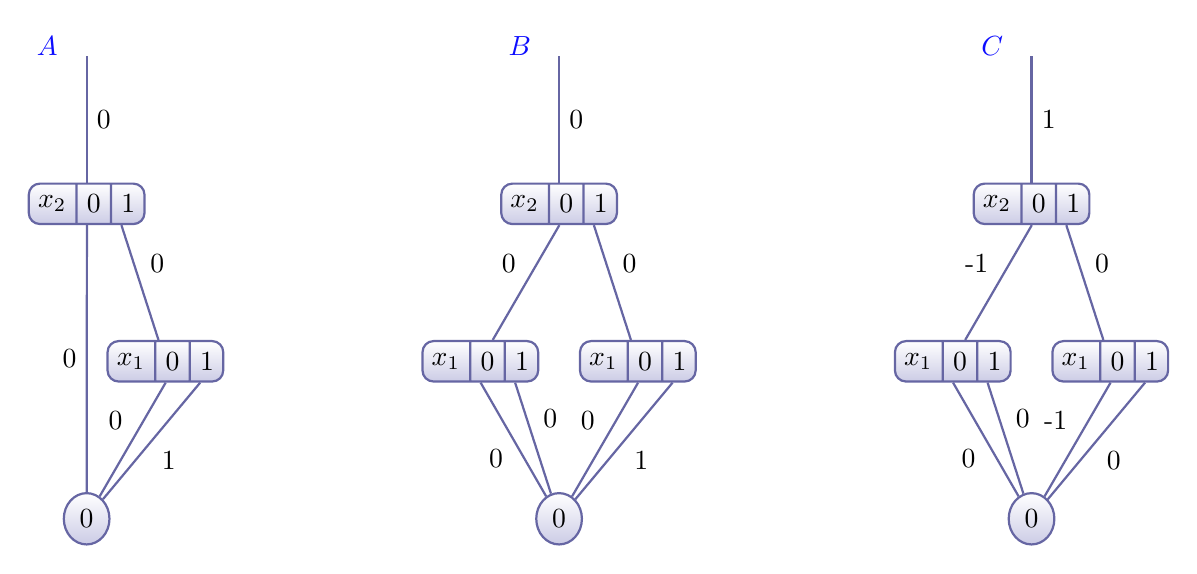
\begin{tikzpicture}
  [yscale=2, auto]
  \begin{scope}
    \node [comment, xshift=-0.5cm]   at ( 0, 3) {$A$};

    \node                 (top)      at ( 0, 3) {};
    \node [mdd node=3]    (l2n0)     at ( 0, 2) {$x_2$\nodepart{two}0\nodepart{three}1};
    \node [mdd node=3]    (l1n1)     at ( 1, 1) {$x_1$\nodepart{two}0\nodepart{three}1};
    \node [terminal node] (terminal) at ( 0, 0) {0};
    
    \draw [regular edge]  (top)                      to node        {0} (l2n0);
    \draw [regular edge]  (l2n0.two   |- l2n0.south) to node [swap] {0} (terminal);
    \draw [regular edge]  (l2n0.three |- l2n0.south) to node        {0} (l1n1);
    \draw [regular edge]  (l1n1.two   |- l1n1.south) to node [swap] {0} (terminal);
    \draw [regular edge]  (l1n1.three |- l1n1.south) to node        {1} (terminal);
  \end{scope}
  
  \begin{scope}[xshift=6cm]
    \node [comment, xshift=-0.5cm]    at ( 0, 3) {$B$};
    
    \node                 (top')      at ( 0, 3) {};
    \node [mdd node=3]    (l2n0')     at ( 0, 2) {$x_2$\nodepart{two}0\nodepart{three}1};
    \node [mdd node=3]    (l1n0')     at (-1, 1) {$x_1$\nodepart{two}0\nodepart{three}1};
    \node [mdd node=3]    (l1n1')     at ( 1, 1) {$x_1$\nodepart{two}0\nodepart{three}1};
    \node [terminal node] (terminal') at ( 0, 0) {0};
    
    \draw [regular edge]  (top')                       to node        {0} (l2n0');
    \draw [regular edge]  (l2n0'.two   |- l2n0'.south) to node [swap] {0} (l1n0');
    \draw [regular edge]  (l2n0'.three |- l2n0'.south) to node        {0} (l1n1');
    \draw [regular edge]  (l1n0'.two   |- l1n0'.south) to node [swap] {0} (terminal');
    \draw [regular edge]  (l1n0'.three |- l1n0'.south) to node        {0} (terminal');
    \draw [regular edge]  (l1n1'.two   |- l1n1'.south) to node [swap] {0} (terminal');
    \draw [regular edge]  (l1n1'.three |- l1n1'.south) to node        {1} (terminal');
  \end{scope}
  \begin{scope}[xshift=12cm]
    \node [comment, xshift=-0.5cm]    at ( 0, 3) {$C$};
    
    \node                 (top')      at ( 0, 3) {};
    \node [mdd node=3]    (l2n0')     at ( 0, 2) {$x_2$\nodepart{two}0\nodepart{three}1};
    \node [mdd node=3]    (l1n0')     at (-1, 1) {$x_1$\nodepart{two}0\nodepart{three}1};
    \node [mdd node=3]    (l1n1')     at ( 1, 1) {$x_1$\nodepart{two}0\nodepart{three}1};
    \node [terminal node] (terminal') at ( 0, 0) {0};
    
    \draw [regular edge]  (top')                       to node        { 1} (l2n0');
    \draw [regular edge]  (l2n0'.two   |- l2n0'.south) to node [swap] {-1} (l1n0');
    \draw [regular edge]  (l2n0'.three |- l2n0'.south) to node        { 0} (l1n1');
    \draw [regular edge]  (l1n0'.two   |- l1n0'.south) to node [swap] { 0} (terminal');
    \draw [regular edge]  (l1n0'.three |- l1n0'.south) to node        { 0} (terminal');
    \draw [regular edge]  (l1n1'.two   |- l1n1'.south) to node [swap] {-1} (terminal');
    \draw [regular edge]  (l1n1'.three |- l1n1'.south) to node        { 0} (terminal');
  \end{scope}
\end{tikzpicture}
  
  \caption{Three EVMDDs on group $(\Z, +)$ representing the same function $f:\{0, 1\}^2\rightarrow\Z, (x_2, x_1)\mapsto x_2\times x_1$.}
\label{figure-reduced}
\end{figure}

\begin{mydefinition}
Given a node $n$ with $\level{n} = k$ and $i_k,\ldots, i_{k'} \in S_k \times \ldots \times S_{k'}$, we define $n(i_k, \ldots, i_{k'})$
$$
n(i_k,\ldots, i_{k'}) = \left\{
  \begin{array}{ll}
    \val{n[i_k]}&\m{if}\;\level{\node{n[i_k]}} < k'\\
    \val{n[i_k]} * \node{n[i_k]}(i_{\level{\node{n[i_k]}}},\ldots, i_{k'})&\m{if}\;\level{\node{n[i_k]}} \geq k'
  \end{array}
\right.
$$
\end{mydefinition}

This allows the definition of the \emph{represented function} for any EVMDD $A$ as

$$
\begin{array}{lcrcl}
  f&:&S&\rightarrow&G\\
   & &(i_K,\ldots, i_1)&\mapsto&\val{A} * \node{A}(i_{\level{\node{A}}},\ldots, i_1)
\end{array}
$$

In other words, $n(i_k,\ldots, i_{k'})$ is the repetitive application of law $*$
on edge values along the path going down from node $n$ and following directions
given by $(i_k,\ldots, i_{k'})$. Hence $f(i_K,\ldots, i_1)$ is $*$ on a path from
the root to the terminal node of $A$.

In this setup, every EVMDD $A$ represents a function $f:S\rightarrow G$.
The reciprocal is also true: given a function $f$, an EVMDD $A$ representing
$f$ can be built by setting the values of all edges of $A$ to the identity element $e$
of $G$, except those pointing to the terminal node, which take proper values
$f(i_k,\ldots, i_1)$ according to the incoming path leading to it.

\begin{myexample}
In Figure~\vref{figure-reduced}, the EVMDD $B$ is built
from $f:\{0, 1\}^2\rightarrow\Z, (x_2, x_1)\mapsto x_2\times x_1$. according to the method explained above.
\end{myexample}

\begin{mydefinition}\label{definition-reduced}
A redundant node $n$ has all outgoing edges identical
$$
\forall i, j \in S_{\level{n}}\,.\; n[i] = n[j]
$$
A \emph{reduced} EVMDD contains no duplicate or redundant nodes.
\end{mydefinition}

\begin{mydefinition}\label{definition-quasi-reduced}
A \emph{quasi-reduced} EVMDD contains no duplicate nodes and all internal nodes $n$ 
have all the descendants on the level below
$$
\forall i \in S_{\level{n}}\,.\; \level{\node{n[i]}} = \level{n}-1
$$
\end{mydefinition}

From any EVMDD $A$, we can build a reduced EVMDD representing the same function
by just deleting nodes with all children identical and redirecting the incoming edges to its unique descendant.
Similarly, from any EVMDD $A$, a quasi reduced EVMDD can be built by adding
nodes with all children identical on edges spanning multiple levels.

\begin{myexample}
In Figure~\vref{figure-reduced} $A$ is reduced, whereas $B$ and $C$ are quasi-reduced.
\end{myexample}

For the sake of simplicity we will only consider quasi-reduced EVMDDs in the following discussion. However, proofs and algorithms for the reduced version are very similar, only slightly more evolved in order to deal with edges skipping levels. We will turn back to reduced EVMDDs only for implementation since they are never larger in size than their quasi-reduced counterpart, hence could have more efficient algorithms.

As can be seen in the previous example, even when restricting to quasi-reduced diagrams,
the EVMDD representation of a function $f$ may not be uniquely defined.

\begin{mydefinition}
A \emph{canonical node} is either the terminal node or a node $n$ such that $\val{n[0]} = e$.

A \emph{canonical EVMDD} is an EVMDD in which all nodes are canonical.
\end{mydefinition}

It can be proved that for every function $f$, there exists a unique
canonical EVMDD representing it~\cite{FMCAD2002}.

In the following, EVMDDs are assumed to be canonical.

%-------------------------------------------------------
\subsection{Extensions%
  \label{subsection-extensions}}

EVMDDs can be used even when the algebraic structure is not a group.
\cite{FMCAD2002} offers a canonization rule for $\N\cup \{+\infty\}$ and
$(\Z, \times)$ can be handled with the canonization rule
``${\rm gcd}\{\val{n[i]}\;|\; i \in S_{\level{n}}\} = 1$ and
$(\val{n[0]},\ldots, \val{n[n_{\level{n}}]}) \geq_{\rm lex} 0$''.

It is also interesting to notice that EVMDDs are just a generalization
of binary decision diagrams with complemented edges, as presented for example
in~\cite{Brace1990}. Indeed, they are edge-valued diagrams on $G = \Z/2\Z$
and complemented (respectively not complemented) edges corresponding to value $1$ (respectively $0$).

%=======================================================
\section{EVMDDs compared to MTMDDs}

MTBDDs are commonly used in model checking to build the transition 
relation of discrete-state systems. In this section we show that EVMDDs 
are at least as suited for that purpose and oftentimes significantly 
better. In the remainder of this section, we pick, often without loss of 
generality, $(G, *) = (\Z, +)$.

%-------------------------------------------------------
\subsection{Space Complexity}

As stated in section 2.2.6 of~\cite{Lai1996}.

\begin{mytheorem}
  \label{theorem-evmdd-smaller-than-add}
  For any function $f$, the number of nodes of the EVMDD representing $f$
  is at most the number of nodes of the MTMDD representing the same function $f$. 
\end{mytheorem}

\Proof{
  Let $A$ be the MTMDD representing $f$. From $A$ we construct the EVMDD (not in canonical form) $A_0$ by replacing each edge from level $1$ to a terminal with value $v$ with an edge with value $v$ to the unique terminal node $0$ and associating value $0$ to all other edges (see Figure~\vref{figure-A-to-A0} for an example)\footnote{This process is similar to the one used in section~\vref{subsection-definition} to prove that every function can be represented by an EVMDD.}.
  \begin{figure}[htbp]
    \centering
        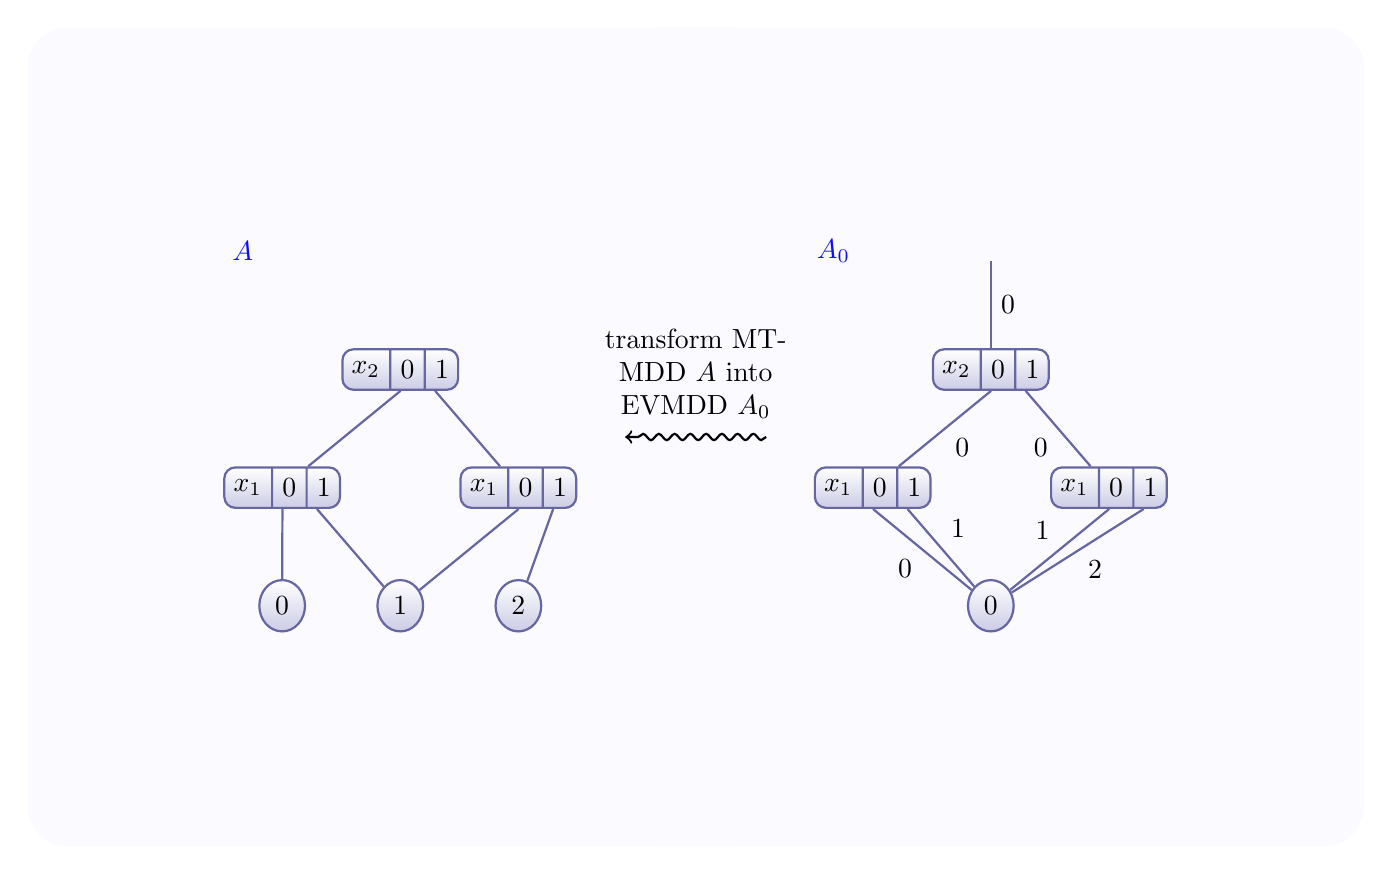
\begin{tikzpicture}
      [scale=1.5, auto]
      \begin{scope}
        \node [comment, xshift=-0.5cm]    at (-1, 3) {$A$};

        \node                 (top)       at ( 0, 3) {};
        \node [mdd node=3]    (l2n0)      at ( 0, 2) {$x_2$\nodepart{two}0\nodepart{three}1};
        \node [mdd node=3]    (l1n0)      at (-1, 1) {$x_1$\nodepart{two}0\nodepart{three}1};
        \node [mdd node=3]    (l1n1)      at ( 1, 1) {$x_1$\nodepart{two}0\nodepart{three}1};
        \node [terminal node] (terminal0) at (-1, 0) {0};
        \node [terminal node] (terminal1) at ( 0, 0) {1};
        \node [terminal node] (terminal2) at ( 1, 0) {2};

        \draw [regular edge]  (l2n0.two   |- l2n0.south) to (l1n0);
        \draw [regular edge]  (l2n0.three |- l2n0.south) to (l1n1);
        \draw [regular edge]  (l1n0.two   |- l1n0.south) to (terminal0);
        \draw [regular edge]  (l1n0.three |- l1n0.south) to (terminal1);
        \draw [regular edge]  (l1n1.two   |- l1n1.south) to (terminal1);
        \draw [regular edge]  (l1n1.three |- l1n1.south) to (terminal2);
      \end{scope}

      \begin{scope}[xshift=5cm]
        \node [comment, xshift=-0.5cm]    at (-1, 3) {$A_0$};

        \node                 (top')      at ( 0, 3) {};
        \node [mdd node=3]    (l2n0')     at ( 0, 2) {$x_2$\nodepart{two}0\nodepart{three}1};
        \node [mdd node=3]    (l1n0')     at (-1, 1) {$x_1$\nodepart{two}0\nodepart{three}1};
        \node [mdd node=3]    (l1n1')     at ( 1, 1) {$x_1$\nodepart{two}0\nodepart{three}1};
        \node [terminal node] (terminal') at ( 0, 0) {0};


        \draw [regular edge]  (top')                       to node        {0} (l2n0');
        \draw [regular edge]  (l2n0'.two   |- l2n0'.south) to node        {0} (l1n0');
        \draw [regular edge]  (l2n0'.three |- l2n0'.south) to node [swap] {0} (l1n1');
        \draw [regular edge]  (l1n0'.two   |- l1n0'.south) to node [swap] {0} (terminal');
        \draw [regular edge]  (l1n0'.three |- l1n0'.south) to node        {1} (terminal');
        \draw [regular edge]  (l1n1'.two   |- l1n1'.south) to node [swap] {1} (terminal');
        \draw [regular edge]  (l1n1'.three |- l1n1'.south) to node        {2} (terminal');
      \end{scope}

      \begin{pgfonlayer}{background}
        \node [scale=2] (r1) [diagram background, fit=(top)(l2n0)(l1n0)(l1n1)(terminal0)(terminal1)(terminal2)] {};
        \node [scale=2] (r2) [diagram background, fit=(top')(l2n0')(l1n0')(l1n1')(terminal')] {};
      \end{pgfonlayer}

      \draw [shorten >=1mm,-to,thick,decorate,
      decoration={snake,amplitude=.4mm,segment length=2mm,
        pre=moveto,pre length=1mm,post length=2mm}]
      (r1) -- (r2) node [above=1mm,midway,text width=3cm,text centered]
      {transform MTMDD $A$ into EVMDD $A_0$};
    \end{tikzpicture}

    \caption{Building the EVMDD $A_0$ (right) from MTMDD $A$ (left)}
    \label{figure-A-to-A0}
  \end{figure}
  Then, we iteratively compute the EVMDD $A_k$, for each $k$ from $1$ to $n$, through the following process:
  \begin{itemize}
  \item for each node $n$ at level $k$, subtract $\val{n[0]}$ from all outgoing edges and add this value to all incoming edges;
  \item merge all duplicate nodes at level $k$ (by duplicate nodes we mean two nodes having edges $x_i$ holding same value and pointing to same children for each $i$ in the range of variable $x_k$).
  \end{itemize}
  See Figure~\vref{figure-A0-to-A1} for an example.

  \begin{figure}[htbp]
    \centering
        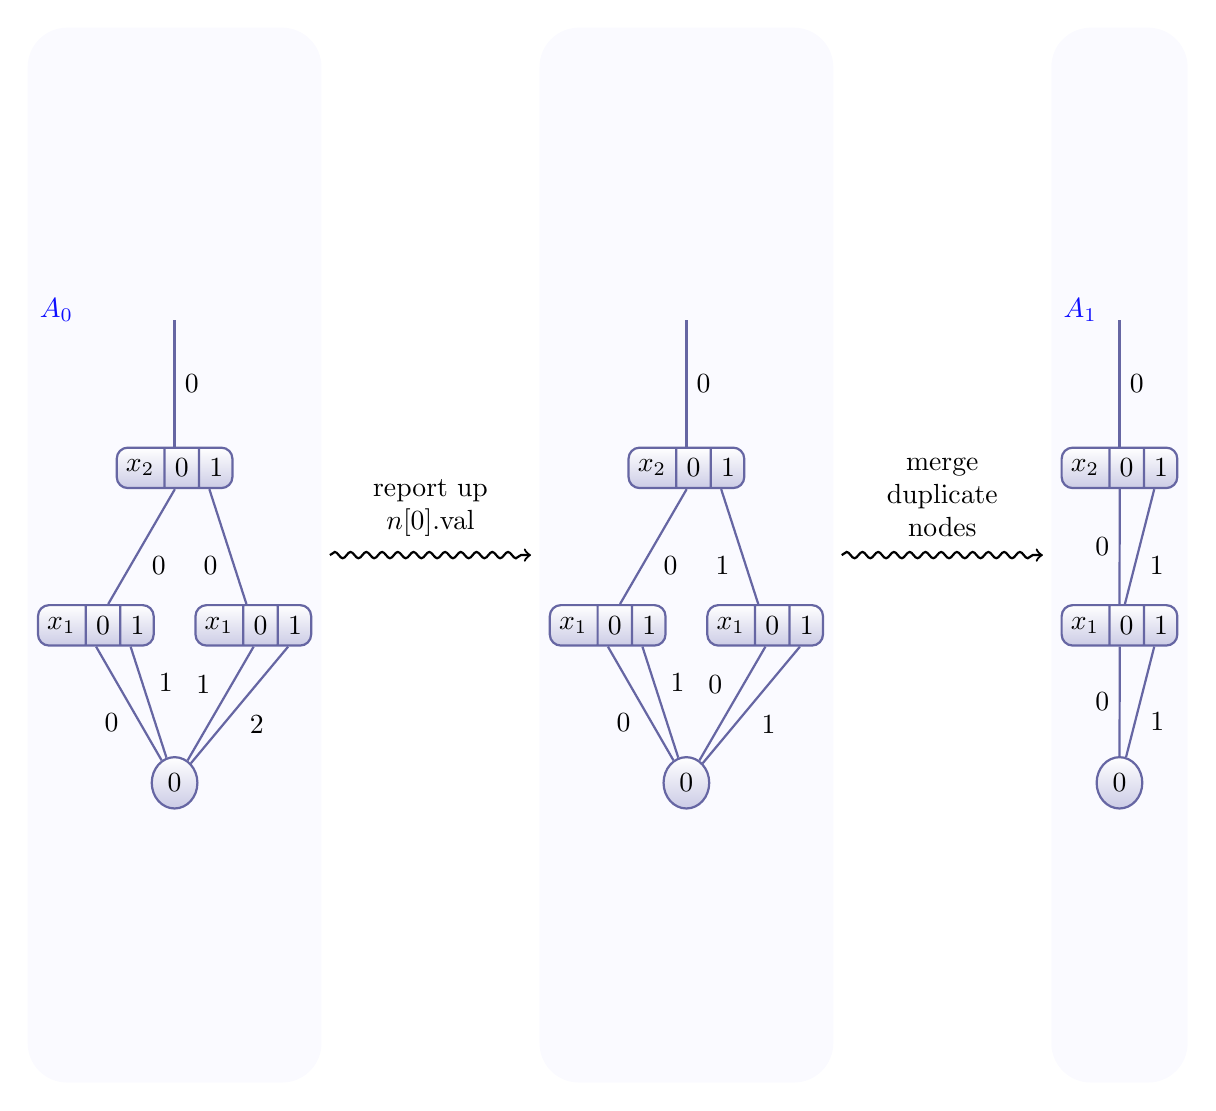
\begin{tikzpicture}
      [yscale=2, auto]
      \begin{scope}
        \node [comment, xshift=-0.5cm]   at (-1, 3) {$A_0$};

        \node                 (top)      at ( 0, 3) {};
        \node [mdd node=3]    (l2n0)     at ( 0, 2) {$x_2$\nodepart{two}0\nodepart{three}1};
        \node [mdd node=3]    (l1n0)     at (-1, 1) {$x_1$\nodepart{two}0\nodepart{three}1};
        \node [mdd node=3]    (l1n1)     at ( 1, 1) {$x_1$\nodepart{two}0\nodepart{three}1};
        \node [terminal node] (terminal) at ( 0, 0) {0};

        \draw [regular edge]  (top)                      to node        {0} (l2n0);
        \draw [regular edge]  (l2n0.two   |- l2n0.south) to node        {0} (l1n0);
        \draw [regular edge]  (l2n0.three |- l2n0.south) to node [swap] {0} (l1n1);
        \draw [regular edge]  (l1n0.two   |- l1n0.south) to node [swap] {0} (terminal);
        \draw [regular edge]  (l1n0.three |- l1n0.south) to node        {1} (terminal);
        \draw [regular edge]  (l1n1.two   |- l1n1.south) to node [swap] {1} (terminal);
        \draw [regular edge]  (l1n1.three |- l1n1.south) to node        {2} (terminal);
      \end{scope}

      \begin{scope}[xshift=6.5cm]
        \node                 (top')      at ( 0, 3) {};
        \node [mdd node=3]    (l2n0')     at ( 0, 2) {$x_2$\nodepart{two}0\nodepart{three}1};
        \node [mdd node=3]    (l1n0')     at (-1, 1) {$x_1$\nodepart{two}0\nodepart{three}1};
        \node [mdd node=3]    (l1n1')     at ( 1, 1) {$x_1$\nodepart{two}0\nodepart{three}1};
        \node [terminal node] (terminal') at ( 0, 0) {0};

        \draw [regular edge]  (top')                       to node        {0} (l2n0');
        \draw [regular edge]  (l2n0'.two   |- l2n0'.south) to node        {0} (l1n0');
        \draw [regular edge]  (l2n0'.three |- l2n0'.south) to node [swap] {1} (l1n1');
        \draw [regular edge]  (l1n0'.two   |- l1n0'.south) to node [swap] {0} (terminal');
        \draw [regular edge]  (l1n0'.three |- l1n0'.south) to node        {1} (terminal');
        \draw [regular edge]  (l1n1'.two   |- l1n1'.south) to node [swap] {0} (terminal');
        \draw [regular edge]  (l1n1'.three |- l1n1'.south) to node        {1} (terminal');
      \end{scope}

      \begin{scope}[xshift=12cm]
        \node [comment, xshift=-0.5cm]     at ( 0, 3) {$A_1$};

        \node                 (top'')      at ( 0, 3) {};
        \node [mdd node=3]    (l2n0'')     at ( 0, 2) {$x_2$\nodepart{two}0\nodepart{three}1};
        \node [mdd node=3]    (l1n0'')     at ( 0, 1) {$x_1$\nodepart{two}0\nodepart{three}1};
        \node [terminal node] (terminal'') at ( 0, 0) {0};

        \draw [regular edge]  (top'')                        to node        {0} (l2n0'');
        \draw [regular edge]  (l2n0''.two   |- l2n0''.south) to node [swap] {0} (l1n0'');
        \draw [regular edge]  (l2n0''.three |- l2n0''.south) to node        {1} (l1n0'');
        \draw [regular edge]  (l1n0''.two   |- l1n0''.south) to node [swap] {0} (terminal'');
        \draw [regular edge]  (l1n0''.three |- l1n0''.south) to node        {1} (terminal'');
      \end{scope}

      \begin{pgfonlayer}{background}
        \node [yscale=2] (r1) [diagram background, fit=(top)(l2n0)(l1n0)(l1n1)(terminal)] {};
        \node [yscale=2] (r2) [diagram background, fit=(top')(l2n0')(l1n0')(l1n1')(terminal')] {};
        \node [yscale=2] (r3) [diagram background, fit=(top'')(l2n0'')(l1n0'')(terminal'')] {};
      \end{pgfonlayer}

      \draw [shorten >=1mm,-to,thick,decorate,
      decoration={snake,amplitude=.4mm,segment length=2mm,
        pre=moveto,pre length=1mm,post length=2mm}]
      (r1) -- (r2) node [above=1mm,midway,text width=2cm,text centered]
      {report up $\val{n[0]}$};
      \draw [shorten >=1mm,-to,thick,decorate,
      decoration={snake,amplitude=.4mm,segment length=2mm,
        pre=moveto,pre length=1mm,post length=2mm}]
      (r2) -- (r3) node [above=1mm,midway,text width=2cm,text centered]
      {merge duplicate nodes};
    \end{tikzpicture}
    
    \caption{Constructing EVMDD $A_1$ (right) from EVMDD $A_0$ (left)}
    \label{figure-A0-to-A1}
  \end{figure}

To prove that $A_k$ and $A$ represent the same function, it is 
sufficient to see that $A$ and $A_0$ represent the same function and that 
the iterative transformation preserves the sum of values on any path $(i_K, \ldots, i_1)$ from 
the root of the diagram to the unique terminal node (plus the value
of the root's incoming edge)
$$
\val{A_k}+\node{A_k}(i_K, \ldots, i_1) = \val{A_{k-1}}+\node{A_{k-1}}(i_K, \ldots, i_1)
$$

Since $A_K$ is in canonical form and since for each $k$, the number of nodes of 
$A_k$ is at most the number of nodes of $A_{k-1}$, 
we can conclude that the size of an EVMDD is never larger than that of the corresponding MTMDD.
}%\end{proof}

This doesn't prove that EVMDDs always require less memory than MTMDDs since
they need extra space to store the edge values, but no worse than up to a small factor
\footnote{Usually $2$, assuming that edge values are as
big as node pointers.}. On the other hand, EVMDDs can be exponentially better than
MTMDD in some cases. For example, the function
$$
\begin{array}{rcl}
  \{0, B-1\}^K&\rightarrow&\Z\\
  (i_K,\ldots, i_1)&\mapsto&\sum_{k=1}^{K} i_k B^{k-1}
\end{array}
$$
where ($B \geq 2$),
requires $\frac{B^{K+1}-1}{B-1}$ nodes in its MTMDD representation%
\footnote{Since all terminal values are distinct.}
whereas it can be represented as an EVMDD with only $K+1$ nodes%
\footnote{More generally, any linear function requires only
one node per level in its EVMDD representation.}.

%-------------------------------------------------------
\subsection{Time complexity%
  \label{subsection-time-complexity}}

What makes decision diagrams a useful data structure
for symbolic model-checking is not only their space efficiency
but the ability to efficiently compute common operations.

Section 2 of~\cite{Clarke1995} gives an algorithm to compute any
binary operation on MTBDDs. The \emph{apply} algorithm can be
easily generalized to MDDs for any
$n$-ary operator $\square_n$. It computes its result in time
$\O{\prod_{i=1}^n |f_i|}$, where $|f_i|$ is the size of MTMDD representing
operand $i$ (in nodes).

Section 2.2 of~\cite{Lai1996} gives the equivalent Algorithm~\vref{algorithm-generic} for
edge-valued decision diagrams.
\begin{algorithm}[htbp]
  \caption{computes any binary operation $\square_2$ on EVMDDs $\edge{v}{n}$ and $\edge{v'}{n'}$}
  \label{algorithm-generic}
  \begin{algorithmic}
    \item[apply($\square_2$ : edge $*$ edge $\rightarrow$ edge, $\edge{v}{n}$ : edge, $\edge{v'}{n'}$ : edge) : edge]
    \STATE $k \gets \level{n}$ \COMMENT{$= \level{n'}$ since EVMDDs are quasi-reduced}
    \BLANK
    \STATE \COMMENT{base case}
    \IF{$k = 0$}
      \RETURN $\edge{v \,\square_2\, v'}{t}$ \COMMENT{$t$ is the unique terminal node}
    \ENDIF
    \BLANK
    \STATE \COMMENT{lookup in cache}
    \IF{CacheFind($\square_2$, $\edge{v}{n}$, $\edge{v'}{n'}$, $\edge{m}{r}$)}
      \RETURN $\edge{m}{r}$
    \ENDIF
    \BLANK
    \STATE $r \gets$ NewNode($k$)
    \FOR{$i = 0$ \textbf{to} $n_k-1$}
      \STATE $r[i] \gets$ apply($\square_2$, $\edge{v+\val{n[i]}}{\node{n[i]}}$, $\edge{v'+\val{n'[i]}}{\node{n'[i]}}$)
    \ENDFOR
    \STATE $m \gets \val{r[0]}$
    \FOR{$i = 0$ \textbf{to} $n_k-1$}
      \STATE $\val{r[i]} \gets \val{r[i]} - m$
    \ENDFOR 
    \BLANK
    \STATE \COMMENT{check if a node identical to $r$ already exists}
    \STATE $r \gets$ FindOrAdd($r$)
    \BLANK
    \STATE \COMMENT{save result in cache}
    \STATE CacheInsert($\square_2$, $\edge{v}{n}$, $\edge{v'}{n'}$, $\edge{m}{r}$)
    \BLANK
    \RETURN $\edge{m}{r}$
  \end{algorithmic}
\end{algorithm}
This is the binary version, but $n$-ary one is very similar for any $n \in \N^*$.

As stated in section 2.2.6 of~\cite{Lai1996}

\begin{mytheorem}
\label{th:rec-calls}
The number of recursive calls of the above \emph{apply} algorithm is the same for MTMDDs
and for EVMDDs representing the same functions.
\end{mytheorem}

\begin{mylemma}
  \label{lemma-n-k-1}

Two paths $(i_K, \ldots, i_{k+1})$ and $(j_K, \ldots, j_{k+1})$ lead to 
the same node in $A$
$$
\node{A}[i_K, \ldots, i_{k+1}] = \node{A}[j_K, \ldots, j_{k+1}]
$$
if and only if they lead to the same node in $A_{k-1}$
$$
\node{A_{k-1}}[i_K, \ldots, i_{k+1}] = A_{k-1}[j_K, \ldots, j_{k+1}]
$$
\end{mylemma}

\Proof{
  $A$ and $A_{k-1}$ are identical from level $k+1$ to level $K$.
}%\end{proof}

\begin{mylemma}
  \label{lemma-n-k}
  Two paths $(i_K, \ldots, i_{k+1})$ and $(j_K, \ldots, j_{k+1})$ lead to the same node in $A_K$ with the same value
$$
\begin{array}{ll}
&\node{A_K}[i_K, \ldots, i_{k+1}] = \node{A_K}[j_K, \ldots, j_{k+1}]\\
\;\;\;\m{and}\;\;\;&
\node{A_K}(i_K, \ldots, i_{k+1}) = \node{A_K}(j_K, \ldots, j_{k+1})
\end{array}
$$
if and only if they lead to the same node in $A_k$ with the same value
$$
\begin{array}{ll}
&\node{A_k}[i_K, \ldots, i_{k+1}] = \node{A_k}[j_K, \ldots, j_{k+1}]\\
\;\;\;\m{and}\;\;\;&
\node{A_k}(i_K, \ldots, i_{k+1}) = \node{A_k}(j_K, \ldots, j_{k+1})
\end{array}
$$
\end{mylemma}

\Proof{
  First, let us prove by induction on $l$, from $k$ to $K$, that:
$$
\begin{array}{ll}
&\node{A_k}[i_K, \ldots, i_{k+1}] = \node{A_l}[i_K, \ldots, i_{k+1}]\\
\;\;\;\m{and}\;\;\;&
\val{A_k}+\node{A_k}(i_K, \ldots, i_{k+1}) = \val{A_l}+\node{A_l}(i_K, \ldots, i_{k+1})
\end{array}
$$
  \begin{itemize}
  \item for $l = k$, the property trivially holds;
  \item if the property holds for a value of $l$ between $k$ and $K-1$, it still holds for $l+1$, since the computation of $A_{l+1}$ from $A_l$ can only merge duplicate nodes at level $l+1 \ge k+1$.
  \end{itemize}
}%\end{proof}

\Proof{[Theorem~\ref{th:rec-calls}]
  We show the proof for the unary version of the algorithm.
  Proofs for other versions are similar, only a bit more verbose.

If we do not take into consideration the caches, the two algorithms are obviously equivalent so 
what we need to prove is that a cache hit occurs in the EVMDD \emph{apply} 
algorithm with diagram $A_K$ if and only if it occurs in the MTMDD algorithm 
with diagram $A$. In other words, we have to prove for every two paths 
$(i_K, \ldots, i_{k+1})$ and $(j_K, \ldots, j_{k+1})$ that they lead to the 
same node in $A$
$$
\node{A}[i_K, \ldots, i_{k+1}] = \node{A}[j_K, \ldots, j_{k+1}]
$$
if and only if they reach the same node in $A_K$ with the same value:
$$
\begin{array}{ll}
&\node{A_K}[i_K, \ldots, i_{k+1}] = \node{A_K}[j_K, \ldots, j_{k+1}]\\
\;\;\;\m{and}\;\;\;&
\node{A_K}(i_K, \ldots, i_{k+1}) = \node{A_K}(j_K, \ldots, j_{k+1})
\end{array}
$$

Therefore, from lemmas \vref{lemma-n-k-1} and \vref{lemma-n-k} it remains to prove 
that two paths $(i_K, \ldots, i_{k+1})$ and $(j_K, \ldots, j_{k+1})$ lead to 
the same node in $A_{k-1}$
\begin{equation}
\label{eqn-k-1}
\node{A_{k-1}}[i_K, \ldots, i_{k+1}] = \node{A_{k-1}}[j_K, \ldots, j_{k+1}]
\end{equation}
if and only if they reach the same node in $A_k$ with the same value:
\begin{equation}
\label{eqn-k}
\begin{array}{ll}
&\node{A_k}[i_K, \ldots, i_{k+1}] = \node{A_k}[j_K, \ldots, j_{k+1}]\\
\;\;\;\m{and}\;\;\;&
\node{A_k}(i_K, \ldots, i_{k+1}) = \node{A_k}(j_K, \ldots, j_{k+1})
\end{array}
\end{equation}

\begin{itemize}

\item Let us prove that (\ref{eqn-k-1}) implies (\ref{eqn-k}).
The first part of (\ref{eqn-k}) is obvious: if two paths lead to the same node before
merging, this still holds after merging. Second part is slightly more complex.
Indeed, $\node{A_k}(i_K, \ldots, i_{k+1})$ is just the value attached to edge $i_{k+1}$ of node
$\node{A_k}[i_K, \ldots, i_{k+2}]$ since all other edges hold value $0$. This value
is the one reported up when constructing $A_k$ from $A_{k-1}$ for 
node $\node{A_k}[i_K, \ldots, i_{k+1}] = \node{A_k}[j_K, \ldots, j_{k+1}]$ so it is the
same for $\node{A_k}(j_K, \ldots, j_{k+1})$, which is the second part of (\ref{eqn-k}).

\item In the other direction: (\ref{eqn-k}) implies (\ref{eqn-k-1}). \\
If (\ref{eqn-k}) holds then $\node{A_{k-1}}[i_K, \ldots, i_{k+1}]$ and
$\node{A_{k-1}}[j_K,\ldots, j_{k+1}]$ are identical (for if they were not, then (\ref{eqn-k})
does not hold on $A_k$ computed from $A_{k-1}$). Hence (\ref{eqn-k-1}), since
$A_{k-1}$ doesn't contain any duplicate at level $k$.

\end{itemize}
}%\end{proof}

In conclusion, EVMDD computations are at least not slower than the MTMDD equivalent.
However, particular operators $\square_n$ may enable much better algorithms on EVMDDs.

%.......................................................
\subsubsection{Addition of Constant: EVMDD $+ c$}

Adding a constant $c$ to an EVMDD $\edge{v}{n}$
is just computing $\edge{c+v}{n}$, which can be done
in constant time.

%.......................................................
\subsubsection{Multiplication with Scalar: EVMDD $\times c$}

As stated in section 2.2.2 of~\cite{Lai1996}, computing
$f \times c$ is just multiplying each edge value
of EVMDD representing $f$ by $c$, which can be done in
time $\O{|f|}$.

%.......................................................
\subsubsection{Addition: EVMDD $+$ EVMDD}

As stated in section 2.2.2 of~\cite{Lai1996},
addition satisfies the property
$$
\edge{v}{n}+\edge{v'}{n'} = (\edge{0}{n}+\edge{0}{n'})+(v+v')
$$
allowing to cache only edges with value $0$, therefore
leading to a slightly modified \emph{apply}, Algorithm~\vref{algorithm-sum}
\begin{algorithm}[htbp]
  \caption{computes sum of EVMDDs $\edge{v}{n}$ and $\edge{v'}{n'}$}
  \label{algorithm-sum}
  \begin{algorithmic}
    \item[plus($\edge{v}{n}$ : edge, $\edge{v'}{n'}$ : edge) : edge]
    \STATE $k \gets \level{n}$ \COMMENT{$= \level{n'}$ since EVMDDs are quasi-reduced}
    \BLANK
    \STATE \COMMENT{base case}
    \IF{$k = 0$}
      \RETURN $\edge{v+v'}{t}$ \COMMENT{$t$ is the unique terminal node}
    \ENDIF
    \BLANK
    \STATE \COMMENT{lookup in cache}
    \IF{CacheFind($+$, $\edge{0}{n}$, $\edge{0}{n'}$, $r$)}
      \RETURN $\edge{v+v'}{r}$
    \ENDIF
    \BLANK
    \STATE $r \gets$ NewNode($k$)
    \FOR{$i = 0$ \textbf{to} $n_k-1$}
      \STATE $r[i] \gets$ plus($n[i]$, $n'[i]$)
    \ENDFOR
    \BLANK
    \STATE \COMMENT{check if a node identical to $r$ already exists}
    \STATE $r \gets$ FindOrAdd($r$)
    \BLANK
    \STATE \COMMENT{save result in cache}
    \STATE CacheInsert($+$, $\edge{v}{n}$, $\edge{v'}{n'}$, $\edge{m}{r}$)
    \BLANK
    \RETURN $\edge{v+v'}{r}$
  \end{algorithmic}
\end{algorithm}
The complexity of the algorithm to compute $f+g$ is $\O{|f|\;|g|}$.

It's also interesting to notice that this algorithm offers
a simple upper bound to the size of the result of an addition
$$
|f+g| \leq |f| \; |g|
$$

%.......................................................
\subsubsection{Remainder and Euclidean Division: EVMDD $\% c$ and EVMDD $/ c$}

As stated in section 2.2.4 of~\cite{Lai1996},
there is no need to cache values equal modulo $c$, hence the complexity of these algorithms is $\O{|f|c}$.
% Algorithms for division and modulo are different (I mean, more than replacing / with %)

%.......................................................
\subsubsection{Minimum and Maximum%
  \label{subsubsection-min-max}}

Per section 2.2.3 of~\cite{Lai1996},
${\rm max}\left\{f(x)\;|\;x \in S\right\}$
and ${\rm min}\left\{f(x)\;|\;x \in S\right\}$
can be easily computed by traversing the graph and caching the result for each node,
hence the complexity is $\O{|f|}$.

%.......................................................
\subsubsection{Multiplication: EVMDD $\times$ EVMDD}

As stated in section 2.2.5 of~\cite{Lai1996},
the result of a multiplication can have an EVMDD
representation of exponential size in terms of the operands.
For example, let $S$ be $\{0, 1\}^K$, $f : (x_K,\ldots, x_1) \mapsto \sum_{k=2}^K x_k2^{k-2}$
and $g : (x_K,\ldots, x_1) \mapsto x_1$, $f$ and $g$ have both an EVMDD representation with $K+1$ nodes
whereas $fg$ needs $2^K$ nodes (here again, we see the importance of variable ordering, putting $x_1$ at top
allows $fg$ to be represented with $2K$ nodes).
Therefore, we cannot expect to find an algorithm with better worst-case
complexity. However, the following equation
$$
\edge{v}{n}\times\edge{v'}{n'} = vv'+v\edge{0}{n'}+v'\edge{0}{n}+\edge{0}{n}\times\edge{0}{n'}
$$
suggests the alternative Algorithm~\vref{algorithm-product}.
\begin{algorithm}[htbp]
  \caption{computes product of EVMDDs $\edge{v}{n}$ and $\edge{v'}{n'}$}
  \label{algorithm-product}
  \begin{algorithmic}
    \item[times($\edge{v}{n}$ : edge, $\edge{v'}{n'}$ : edge) : edge]
    \STATE $k \gets \level{n}$ \COMMENT{$= \level{n'}$ since EVMDDs are quasi-reduced}
    \BLANK
    \STATE \COMMENT{base case}
    \IF{$k = 0$}
      \RETURN $\edge{v\times v'}{t}$ \COMMENT{$t$ is the unique terminal node}
    \ENDIF
    \BLANK
    \STATE \COMMENT{lookup in cache}
    \IF{CacheFind($\times$, $\edge{0}{n}$, $\edge{0}{n'}$, $r$)}
      \RETURN plusc(plus(plus(timesc($\edge{0}{n}$, $v'$), timesc($\edge{0}{n'}$, $v$)), r), $v\times v'$)
    \ENDIF
    \BLANK
    \STATE $r \gets$ NewNode($k$)
    \FOR{$i = 0$ \textbf{to} $n_k-1$}
      \STATE $r[i] \gets$ times($n[i]$, $n'[i]$)
    \ENDFOR
    \BLANK
    \STATE \COMMENT{check if a node identical to $r$ already exists}
    \STATE $r \gets$ FindOrAdd($r$)
    \BLANK
    \STATE \COMMENT{save result in cache}
    \STATE CacheInsert($\times$, $\edge{v}{n}$, $\edge{v'}{n'}$, $\edge{m}{r}$)
    \BLANK
    \RETURN plusc(plus(plus(timesc($\edge{0}{n}$, $v'$), timesc($\edge{0}{n'}$, $v$)), r), $v\times v'$)
  \end{algorithmic}
\end{algorithm}
The first product is an integer multiplication done in constant time.
The next two are multiplications by a constant done in $\O{|f|}$ and $\O{|g|}$, respectively.
The last one is done through recursive calls.
The first addition takes constant time, the second one
takes $\O{|f|\;|g|}$ and produce a result of size at most $|f|\;|g|$,
hence a cost of $\O{|f|\;|g|\;|fg|}$ for the last addition.
The function \texttt{times} is called $\O{|f|\;|g|}$ times, hence a final complexity
of $\O{|f|^2\;|g|^2\;|fg|}$.

Although we were unable to theoretically compare this algorithm to
the generic Algorithm~\vref{algorithm-generic}, it seems to perform
far better in practice when the size of the result is moderate.

%.......................................................
\subsubsection{Relational Operators: EVMDD $< c$}

Relational operators ($<, >, \leq, \geq, =$ and $\neq$) are
used in building transition relations.
Unfortunately, the corresponding operations remain somewhat expensive.
But, as stated in section
2.2.3 of~\cite{Lai1996}, $f < g$ can be computed as $f-g < 0$ and
the operation ``less than constant'' can be greatly improved
as shown in Algorithm~\vref{algorithm-lt} through
the use of min and max, which are easy to compute from section~\vref{subsubsection-min-max}.
\begin{algorithm}[htbp]
  \caption{computes $\edge{v}{n} < c$ for EVMDD $\edge{v}{n}$ and integer $c$}
  \label{algorithm-lt}
  \begin{algorithmic}
    \item[lt($\edge{v}{n}$ : edge, $c$ : int) : edge]
    \STATE $k \gets \level{n}$
    \BLANK
    \STATE \COMMENT{base cases}
    \IF{$c-v \leq {\rm min}(n)$}
      \RETURN $\edge{0}{t}$ \COMMENT{$t$ is the unique terminal node}
    \ENDIF
    \IF{$c-v > {\rm max}(n)$}
      \RETURN $\edge{1}{t}$ \COMMENT{$t$ is the unique terminal node}
    \ENDIF
    \BLANK
    \STATE \COMMENT{lookup in cache}
    \IF{CacheFind($<$, $\edge{0}{n}$, $c-v$, $\edge{m}{r}$)}
      \RETURN $\edge{m}{r}$
    \ENDIF
    \BLANK
    \STATE $r \gets$ NewNode($k$)
    \FOR{$i = 0$ \textbf{to} $n_k-1$}
      \STATE $r[i] \gets$ lt($n[i]$, $c-v$)
    \ENDFOR
    \STATE $m \gets \val{r[0]}$
    \FOR{$i = 0$ \textbf{to} $n_k-1$}
      \STATE $\val{r[i]} \gets \val{r[i]}-m$
    \ENDFOR
    \BLANK
    \STATE \COMMENT{check if a node identical to $r$ already exists}
    \STATE $r \gets$ FindOrAdd($r$)
    \BLANK
    \STATE \COMMENT{save result in cache}
    \STATE CacheInsert($<$, $\edge{0}{n}$, $c-v$, $\edge{m}{r}$)
    \BLANK
    \RETURN $\edge{m}{r}$
  \end{algorithmic}
\end{algorithm}

We also developed Algorithm~\vref{algorithm-alt-lt}, which initially was deemed as ``optimized''.
\begin{algorithm}[htbp]
  \caption{computes $\edge{v}{n} < c$ for EVMDD $\edge{v}{n}$ and integer $c$}
  \label{algorithm-alt-lt}
  \begin{algorithmic}
    \item[lt($\edge{v}{n}$ : edge, $c$ : int) : int $*$ int $*$ edge]
    \STATE $k \gets \level{n}$
    \BLANK
    \STATE \COMMENT{base cases}
    \IF{$c-v \leq {\rm min}(n)$}
      \RETURN $(-\infty, {\rm min}(n), \edge{0}{t})$ \COMMENT{$t$ is the unique terminal node}
    \ENDIF
    \IF{$c-v > {\rm max}(n)$}
      \RETURN $({\rm max}(n)+1, +\infty, \edge{1}{t})$ \COMMENT{$t$ is the unique terminal node}
    \ENDIF
    \BLANK
    \STATE \COMMENT{lookup in cache for an interval $[lb, ub]$ containing $c-v$}
    \IF{CacheFind($<$, $\edge{0}{n}$, $c-v$, $(lb, ub, \edge{m}{r})$)}
      \RETURN $(lb, ub, \edge{m}{r})$
    \ENDIF
    \BLANK
    \STATE $r \gets$ NewNode($k$)
    \STATE $lb \gets -\infty$
    \STATE $ub \gets +\infty$
    \FOR{$i = 0$ \textbf{to} $n_k-1$}
      \STATE $lb', ub', r[i] \gets$ lt($n[i]$, $c-v$)
      \STATE $lb \gets {\rm max}(lb, lb'+\val{n[i]})$
      \STATE $ub \gets {\rm min}(ub, ub'+\val{n[i]})$
    \ENDFOR
    \STATE $m \gets \val{r[0]}$
    \FOR{$i = 0$ \textbf{to} $n_k-1$}
      \STATE $\val{r[i]} \gets \val{r[i]}-m$
    \ENDFOR
    \BLANK
    \STATE \COMMENT{check if a node identical to $r$ already exists}
    \STATE $r \gets$ FindOrAdd($r$)
    \BLANK
    \STATE \COMMENT{save result in cache}
    \STATE CacheInsert($<$, $\edge{0}{n}$, $[lb, ub]$, $(lb, ub, \edge{m}{r})$)
    \BLANK
    \RETURN $(lb, ub, \edge{m}{r})$
  \end{algorithmic}
\end{algorithm}
The idea behind this algorithm is that
for a call $\mathrm{lt}((\_, p), \_)$ returning $(lb, ub, q)$, the 
interval $[lb, ub]$ is the set $\{c \;|\; \forall x.\; 
p\left(x\right) < c \Leftrightarrow 
q\left(x\right) = 1\}$. In other words, $[lb, ub]$
is the exact interval for which the relation $p < .$ is given by $q$.

The later algorithm is theoretically better than the former in that
more cache hits occur. It can even be viewed as optimal in the sense that
it never creates duplicate nodes from a same node of the input EVMDD.
However, in practice, this advantage appears quite small in most cases.
Moreover, in order to implemented it, it requires an ordered cache, such as a search tree,
instead of a simple hash table and the resulting log factor seems to overcome
any advantage.

Algorithms for other relational operators analogous to $<$.

%-------------------------------------------------------
\subsection{Versatility}

The advantages of EVMDDs over MTMDDs come at a price of a slightly reduced versatility.
Both EVMDDs and MTMDDs can be used to represent functions more general than 
arithmetic functions over integers. For MTMDDs, the only restriction is that
the domain and co-domain of the encoded function have to be finite.
However EVMDDs, despite the extensions of section~\vref{subsection-extensions},
also require some algebraic structure. For example, they cannot be directly used
with floats since the sum of two floating point values has to be rounded to
be represented as a floating point value.
In computer arithmetic, \cite{Sasao2009}~encodes floating point functions
through integer EVMDDs of their binary (bit-level) representation. 
Even though space efficient, floating point computations on this representation remain expensive.

Another problem affecting EVMDDs but not MTMDDs is \emph{false overflow}.
Indeed, computers do not operate over $\Z$ proper, but on $\Z/2^{32}\Z$ (for 32bit platforms,
or the equivalent structure for the appropriate size of integers -- 16, 32, 64 bits).
Integer overflow is possible when adding edge values, even when the represented function
may fit within $32$ bits. An example of such an internal overflow
can be seen in figure~\vref{figure-overflow}.
\begin{figure}[htbp]
  \centering
  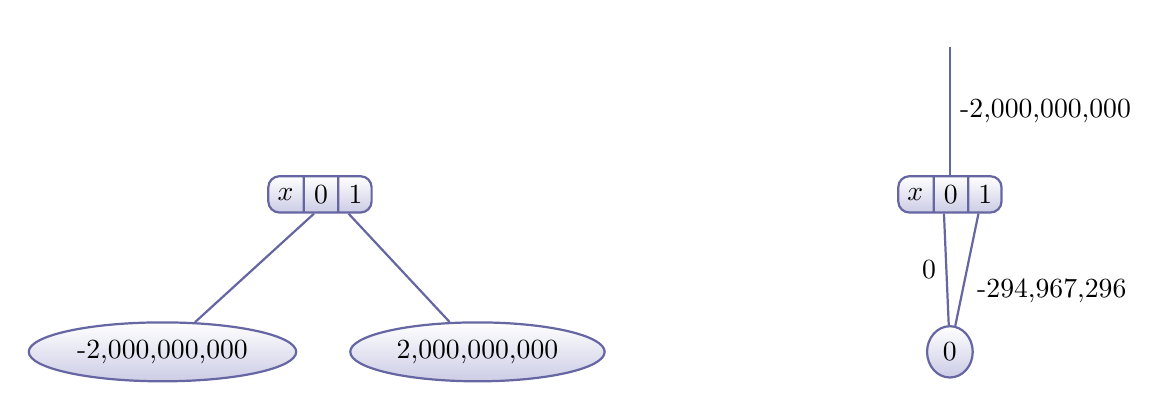
\begin{tikzpicture}
  [scale=2, auto]
  \begin{scope}
    \node                 (top)       at ( 0, 2) {};
    \node [mdd node=3]    (l1n0)      at ( 0, 1) {$x$\nodepart{two}0\nodepart{three}1};
    \node [terminal node] (terminal0) at (-1, 0) {-2,000,000,000};
    \node [terminal node] (terminal1) at ( 1, 0) { 2,000,000,000};
    
    \draw [regular edge]  (l1n0.two   |- l1n0.south) to (terminal0);
    \draw [regular edge]  (l1n0.three |- l1n0.south) to (terminal1);
  \end{scope}
  
  \begin{scope}[xshift=4cm]
    \node                 (top')      at ( 0, 2) {};
    \node [mdd node=3]    (l1n0')     at ( 0, 1) {$x$\nodepart{two}0\nodepart{three}1};
    \node [terminal node] (terminal') at ( 0, 0) {0};
    
    \draw [regular edge]  (top')                       to node        {-2,000,000,000} (l1n0');
    \draw [regular edge]  (l1n0'.two   |- l1n0'.south) to node [swap] {             0} (terminal');
    \draw [regular edge]  (l1n0'.three |- l1n0'.south) to node        {  -294,967,296} (terminal');
  \end{scope}
\end{tikzpicture}
  
  \caption{MTMDD (left) and EVMDD (right) encoding the same function over 32-bit integers,
$f : x \in \{0, 1\} \mapsto 2,000,000,000\times(2x-1)$.}
\label{figure-overflow}
\end{figure}
Since $\Z/2^{32}\Z$ is still an additive group, these overflows are harmless
for addition and multiplication by a constant. The general algorithm from 
section~\vref{subsection-time-complexity} is not affected either, as it applies
operations only on leaf nodes, but this observation no longer holds on 
the other algorithms of this section.
A necessary and sufficient condition on a function $f$ for not having false overflows in 
the corresponding EVMDD is
$$
\begin{array}{l}
\forall k \in \{1,\ldots, K\} \,.\; \forall (i_K,\ldots,i_{k+1}) \in S_K \times \ldots \times S_{k+1} \,.\; \forall i_k \in S_k \,.\;\\
\;\;\; f(i_K,\ldots, i_{k+1}, i_k, 0,\ldots, 0) - f(i_K,\ldots, i_{k+1}, 0, 0,\ldots, 0) \; \m{does not overflow}
\end{array}
$$

%Despite these drawbacks, EVMDDs are very adequate for encoding discrete-state transition relations.

%=======================================================
\section{Implementation}

Symbolic model checkers such as (Nu)SMV\cite{NuSMV} or SAL\cite{SAL}
are based on the library CUDD\cite{CUDD} which offers an efficient
implementation of BDDs and MTBDDs. For state space generation, they
use a plain breadth first search (BFS) algorithm.

Our goal was to implement a new symbolic model checking library featuring
EVMDDs for transition relation construction and saturation\cite{Saturation2001}
for state space generation. We also developed a basic
model checking front-end to test the library and compare it to CUDD.
Binaries for both and model checker sources are available
at \url{http://research.nianet.org/~radu/evmdd/}.

In this section, we discuss some implementation details
before presenting experimental results.

%-------------------------------------------------------
\subsection{Memory Management}

It is well known that model checking can be memory intensive,
making memory management a critical issue when implementing
a decision diagrams library.

The usual addressing scheme of BDD nodes is through pointers.
Here, with MDD, nodes at different levels with different
variable ranges are of different sizes. For that reason, we chose
an index-based addressing scheme $(level, index)$, allowing to allocate nodes
independently at each level.

Decision diagrams algorithms rely heavily on several cache structures.
They are usually implemented as lossy hash tables: upon collision, older entries
are simply discarded. 
We avoided the loss of information by choosing dynamically resizing hash tables with chaining.
The non-lossy caches give slightly faster algorithms at the price
of some additional memory.

Different diagrams often share subgraphs, making explicit freeing
of disconnected sub-diagrams very difficult. Moreover,
symbolic model checking algorithms often produce a large number of temporary
nodes which rapidly become disconnected (also called garbage). 
The easiest way to reclaim
memory is to use some garbage collection procedure.
The most commonly used technique is via reference counting.
This is perfectly suited since diagrams are DAGs, hence avoiding
circular reference, the main drawback of reference counting. 
Instead, we chose to use a simple \emph{mark \& sweep} algorithm that proved
to be both simple and efficient, because it requires minimal book-keeping.
We keep reference counting only as an interface with library users.

%-------------------------------------------------------
\subsection{Encoding the Transition Relation}

We represent the transition relation $T$ as a disjunction
$\bigcup_{e \in E}T_e$ of \emph{events} $e$. Each event $T_e$
is represented as an MDD of high $2K$, with level $2k$
encoding variable $x_k$ before the transition and level $2k-1$
same variable $x_k'$ but after the transition%
\footnote{That is, we consider $T_e$ as a part of
$S \times S = S_K \times S_K \times \ldots \times S_1 \times S_1$.
It is interesting to notice, that $T_e$ does not need to be a function
$S \rightarrow S$, allowing to model non deterministic behaviors.}.

This disjunction representation is well suited for
globally--asynchronous locally--synchronous systems, where
each event encodes some local transition. 
However, we could end up with many events that are just the identity relation for most variables,
The numerous ``identity patterns'' in the MDD are  % in itself, an identity pattern is quite light, but we have lot of them
very expensive to deal with, both in terms of memory usage
and computation time. To avoid this problem, we chose yet another reduction rule of nodes,
different than the two already presented in definitions~\vref{definition-reduced}
and~\vref{definition-quasi-reduced}: the \emph{full-identity reduction} from~\cite{Ciardo2005}.

\begin{figure}[htbp]
  \centering
  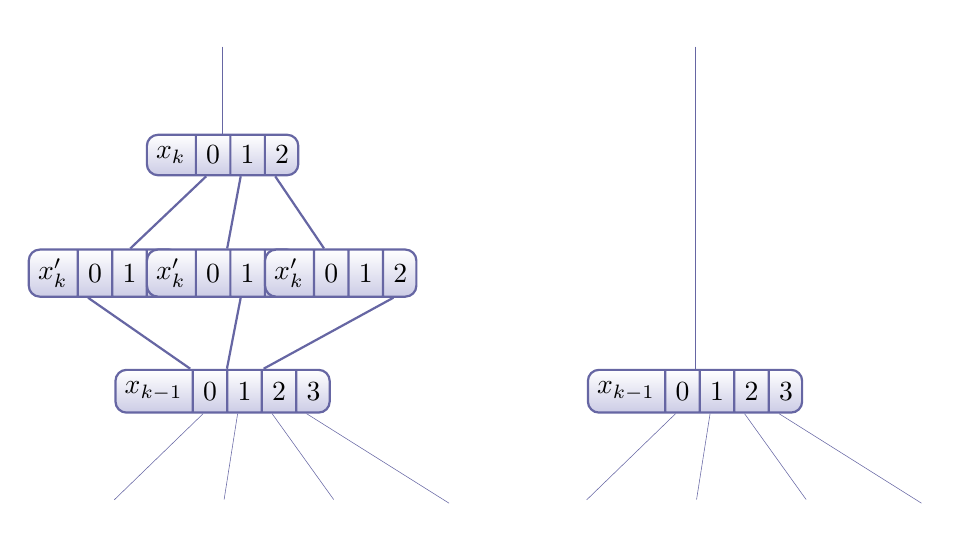
\begin{tikzpicture}
  [xscale=1.5, yscale=1.5, auto]
  \begin{scope}
    \node              (top)     at ( 0, 4) {};
    \node [mdd node=4] (l3n0)    at ( 0, 3) {$x_k$\nodepart{two}0\nodepart{three}1\nodepart{four}2};
    \node [mdd node=4] (l2n0)    at (-1, 2) {$x_k'$\nodepart{two}0\nodepart{three}1\nodepart{four}2};
    \node [mdd node=4] (l2n1)    at ( 0, 2) {$x_k'$\nodepart{two}0\nodepart{three}1\nodepart{four}2};
    \node [mdd node=4] (l2n2)    at ( 1, 2) {$x_k'$\nodepart{two}0\nodepart{three}1\nodepart{four}2};
    \node [mdd node=5] (l1n0)    at ( 0, 1) {$x_{k-1}$\nodepart{two}0\nodepart{three}1\nodepart{four}2\nodepart{five}3};
    \node              (bottom1) at (-1, 0) {};
    \node              (bottom2) at ( 0, 0) {};
    \node              (bottom3) at ( 1, 0) {};
    \node              (bottom4) at ( 2, 0) {};
    
    \draw [outgoing edge] (top)                      to (l3n0);
    \draw [regular edge]  (l3n0.two   |- l3n0.south) to (l2n0);
    \draw [regular edge]  (l3n0.three |- l3n0.south) to (l2n1);
    \draw [regular edge]  (l3n0.four  |- l3n0.south) to (l2n2);
    \draw [regular edge]  (l2n0.two   |- l2n0.south) to (l1n0);
    \draw [regular edge]  (l2n1.three |- l2n1.south) to (l1n0);
    \draw [regular edge]  (l2n2.four  |- l2n2.south) to (l1n0);
    \draw [outgoing edge] (l1n0.two   |- l1n0.south) to (bottom1);
    \draw [outgoing edge] (l1n0.three |- l1n0.south) to (bottom2);
    \draw [outgoing edge] (l1n0.four  |- l1n0.south) to (bottom3);
    \draw [outgoing edge] (l1n0.five  |- l1n0.south) to (bottom4);
  \end{scope}

  \begin{scope}[xshift=4cm]
    \node              (top')     at ( 0, 4) {};
    \node [mdd node=5] (l1n0')    at ( 0, 1) {$x_{k-1}$\nodepart{two}0\nodepart{three}1\nodepart{four}2\nodepart{five}3};
    \node              (bottom1') at (-1, 0) {};
    \node              (bottom2') at ( 0, 0) {};
    \node              (bottom3') at ( 1, 0) {};
    \node              (bottom4') at ( 2, 0) {};
    
    \draw [outgoing edge] (top')                       to (l1n0');
    \draw [outgoing edge] (l1n0'.two   |- l1n0'.south) to (bottom1');
    \draw [outgoing edge] (l1n0'.three |- l1n0'.south) to (bottom2');
    \draw [outgoing edge] (l1n0'.four  |- l1n0'.south) to (bottom3');
    \draw [outgoing edge] (l1n0'.five  |- l1n0'.south) to (bottom4');
  \end{scope}
\end{tikzpicture}
  
  \caption{An identity pattern in a reduced MDD (left) and its identity reduced equivalent (right).}
\label{figure-identity-reduction}
\end{figure}

An example of such an identity pattern and its full-identity
reduction is shown in Figure~\vref{figure-identity-reduction}. 
In this figure, edges leading to terminal $0$ are omitted for clarity.

Table~\vref{table-identity-reduction} shows the execution time
with standard reduction and full-identity reduction rules for the classical model
of dining philosophers.
\begin{table}[htbp]
  \centering
  \begin{tabular}{|r||r|r|}
    \hline
    \multicolumn{1}{|l||}{Model} & standard & full-identity \\
    \multicolumn{1}{|l||}{size}  & (sec) & (sec) \\
    \hline
%      10 & 0.02& 0.00\\
      50 & 0.36& 0.02\\
     100 & 1.68& 0.04\\
     200 & 7.85& 0.07\\
     400 &36.72& 0.20\\
%     500 &  ---& 0.27\\
    1000 &  ---& 0.91\\
    7000 &  ---&37.47\\
    \hline
  \end{tabular}
\vspace*{3mm}
  \caption{Execution time for building the transition relation
using standard and fully-identity reduced MDDs (``---'' means ``out of memory'').}
  \label{table-identity-reduction}
\end{table}
%\vspace*{-5mm}

%-------------------------------------------------------
\subsection{State Space Construction}

For state space construction, we use the Saturation algorithm~\cite{Saturation2001}
instead of the classical breadth first search exploration. This heuristic
often gives spectacular improvements when building the state spaces
of globally--asynchronous locally--synchronous systems.
This is certainly the major source of improvement of our implementation
over existing BDD libraries.

As advised in~\cite{Ciardo2005}, we chose to merge all events $e$
with same topmost affected level%
\footnote{i.e. same value of ${\rm max}\left\{k\;|\;\exists i, j \in S_k\,.\; i \neq j \land (i, j) \in T_e \right\}$}
in the same MDD. The cost of the unions slows down the generation of the transition relation
but generally makes the state space construction up to several times faster.

%-------------------------------------------------------
\subsection{Experimental Results}

Our new model checker comprises $7000$ lines of ANSI-C code for the library
and $4000$ lines for the simple model checker that provides a common interface
to our library and CUDD. Table~\vref{table-results} shows
execution times for finding deadlocks on a suite of classical models.
The search for deadlocks in a deadlock-free system equates to building state space.
Programs to generate all models can be found in the \texttt{examples} directory
of our simple model checker source distribution, available at \url{http://research.nianet.org/~radu/evmdd/}.

We collected the results on a Linux machine with Intel~Core~2 processor, 1.2GHz, 1.5GB of memory.

\IGNORE{
\begin{table}[htb]
  \begin{center}
    \begin{tabular}{|r||r|r|r|}
      \hline
      \multicolumn{1}{|l||}{Model} & \multicolumn{1}{l|}{Reachable} & CUDD & EVMDD \\
      \multicolumn{1}{|l||}{size}  & \multicolumn{1}{l|}{states} & (sec) & (sec) \\
      \hline
      \multicolumn{4}{|l|}{Dining philosophers}\\
      \hline
      100 & $4\times10^{62}$ &    5.15 &    0.04 \\
%      200 & $2\times10^{125}$ & 1493.36 &    0.10 \\
      1000 & $9\times10^{626}$ &   --- &    1.10 \\
      5000 & $6\times10^{3134}$ &   --- &   20.48 \\
      10000 & $4\times10^{6269}$ &   --- &   77.77 \\
      16000 & $2\times10^{10031}$ &   --- &  196.84 \\
      \hline
      \multicolumn{4}{|l|}{Round robin mutual exclusion protocol}\\
      \hline
%      20 & $4\times10^{7}$ &    0.47 &    0.04 \\
      40 & $9\times10^{13}$ &    4.04 &    0.46 \\
      60 & $1\times10^{20}$ &   15.59 &    1.54 \\
      100 & $2\times10^{32}$ &  599.16 &    7.42 \\
      200 & $7\times10^{62}$ &   --- &   75.94 \\
      \hline
      \multicolumn{4}{|l|}{Slotted ring protocol}\\
      \hline
      10 & $8\times10^{9}$ &    1.07 &    0.01 \\
      15 & $1\times10^{15}$ &   13.00 &    0.03 \\
      20 & $2\times10^{20}$ & 1804.48 &    0.04 \\
      100 & $2\times10^{105}$ &   --- &    3.74 \\
%      200 & $8\times10^{211}$ &   --- &   29.73 \\
      300 & $3\times10^{318}$ &   --- &  111.29 \\
      500 & $5\times10^{531}$ &   --- &  505.04 \\
      \hline
    \end{tabular}
    \hspace{1cm}
    \begin{tabular}{|r||r|r||r|r|}
      \hline
      \multicolumn{1}{|l||}{Model} & \multicolumn{1}{l|}{Reachable} & \multicolumn{1}{|l||}{Deadlock} & CUDD & EVMDD \\
      \multicolumn{1}{|l||}{size}  & \multicolumn{1}{l|}{states} & \multicolumn{1}{|l||}{states} & (in s) & (in s) \\
      \hline
      \multicolumn{4}{|l|}{Kanban assembly line}\\
      \hline
      10 & $1\times10^{9}$ &    0.84 &    0.01 \\
      15 & $4\times10^{10}$ &   86.58 &    0.03 \\
      20 & $8\times10^{11}$ &  811.89 &    0.04 \\
      100 & $1\times10^{19}$ &   --- &    3.25 \\
      200 & $3\times10^{22}$ &   --- &   32.31 \\
      400 & $6\times10^{25}$ &   --- &  697.90 \\
      \hline
      \multicolumn{4}{|l|}{Knights problem}\\
      \hline
      5 & $6\times10^{7}$ &  921.95 &    0.30 \\
      7 & $1\times10^{15}$ &   --- &    3.73 \\
      9 & $8\times10^{24}$ &   --- &   47.80 \\
      \hline
      \multicolumn{4}{|l|}{Randomized leader election protocol}\\
      \hline
%      5 & $1\times10^{5}$  &    0.90 &    0.32 \\
%      6 & $2\times10^{6}$  &    4.62 &    1.20 \\
      7 & $2\times10^{7}$   &   23.87 &    3.69 \\
      8 & $3\times10^{8}$   &  176.16 &   10.04 \\
      9 & $5\times10^{9}$   &  810.36 &   24.86 \\
      10 & $6\times10^{10}$ &    ---  &   85.54 \\
      11 & $9\times10^{11}$ &    ---  &  423.41 \\
      \hline
    \end{tabular}
\vspace*{3mm}
    \caption{Execution times for finding deadlocks using our library or CUDD (``---'' means ``more than an hour'').}
    \label{table-results}
  \end{center}
\end{table}
}

{\small
\begin{table}[htb]
  \begin{center}
    \begin{tabular}{|r||r||r|r|}
      \hline
      \multicolumn{1}{|l||}{Model} & \multicolumn{1}{l||}{Reachable} & CUDD & EVMDD \\
      \multicolumn{1}{|l||}{size}  & \multicolumn{1}{l||}{states}  & (sec) & (sec) \\
      \hline
      \multicolumn{4}{|l|}{Dining philosophers}\\
      \hline
      100 & $4\times10^{62}$ &    5.15 &    0.04 \\
      200 & $2\times10^{125}$ & 1493.36 &    0.10 \\
      1000 & $9\times10^{626}$ &   --- &    1.10 \\
%      5000 & $6\times10^{3134}$ &   --- &   20.48 \\
      10000 & $4\times10^{6269}$ &   --- &   77.77 \\
      16000 & $2\times10^{10031}$ &   --- &  196.84 \\
      \hline
      \multicolumn{4}{|l|}{Round robin mutual exclusion protocol}\\
      \hline
%      20 & $4\times10^{7}$ &    0.47 &    0.04 \\
      40 & $9\times10^{13}$ &    4.04 &    0.46 \\
      60 & $1\times10^{20}$ &   15.59 &    1.54 \\
      100 & $2\times10^{32}$ &  599.16 &    7.42 \\
      200 & $7\times10^{62}$ &   --- &   75.94 \\
      \hline
      \multicolumn{4}{|l|}{Slotted ring protocol}\\
      \hline
      10 & $8\times10^{9}$    &    1.07 &    0.01 \\
%      15 & $1\times10^{15}$   &   13.00 &    0.03 \\
      20 & $2\times10^{20}$   & 1804.48 &    0.04 \\
      100 & $2\times10^{105}$ &   --- &    3.74 \\
%      200 & $8\times10^{211}$ &   --- &   29.73 \\
      300 & $3\times10^{318}$ &   --- &  111.29 \\
      500 & $5\times10^{531}$ &   --- &  505.04 \\
      \hline
    \end{tabular}
%    \hspace{1cm}
    \begin{tabular}{|r||r||r|r|r|}
      \hline
      \multicolumn{1}{|l||}{Model} & \multicolumn{1}{l||}{Reachable} & CUDD & EVMDD \\
      \multicolumn{1}{|l||}{size}  & \multicolumn{1}{l||}{states} & (sec) & (sec) \\
      \hline
      \multicolumn{4}{|l|}{Kanban assembly line}\\
      \hline
      10 & $1\times10^{9}$   &    0.84 &    0.01 \\
%      15 & $4\times10^{10}$  &   86.58 &    0.03 \\
      20 & $8\times10^{11}$  &  811.89 &    0.04 \\
      100 & $1\times10^{19}$ &   --- &    3.25 \\
      200 & $3\times10^{22}$ &   --- &   32.31 \\
      400 & $6\times10^{25}$ &   --- &  697.90 \\
      \hline
      \multicolumn{4}{|l|}{Knights problem}\\
      \hline
      5 & $6\times10^{7}$  &  921.95 &    0.30 \\
      7 & $1\times10^{15}$ &   --- &    3.73 \\
      9 & $8\times10^{24}$ &   --- &   47.80 \\
      \hline
      \multicolumn{4}{|l|}{Randomized leader election protocol}\\
      \hline
%      5 & $1\times10^{5}$   &    0.90 &    0.32 \\
      6 & $2\times10^{6}$   &    4.62 &    1.20 \\
      7 & $2\times10^{7}$   &   23.87 &    3.69 \\
      8 & $3\times10^{8}$   &  176.16 &   10.04 \\
      9 & $5\times10^{9}$   &  810.36 &   24.86 \\
      10 & $6\times10^{10}$ &   ---   &   85.54 \\
      11 & $9\times10^{11}$ &   ---   &  423.41 \\
      \hline
    \end{tabular}
\vspace*{3mm}
    \caption{Execution times for finding deadlocks using our library or CUDD (``---'' means ``$>1$hour'').}
    \label{table-results}
  \end{center}
\end{table}
}

Note that using other existing tools, such as NuSMV or SAL on these models, we get execution times of the same order of magnitude as 
with our model checker using CUDD.

Compared to the first implementation of saturation algorithm~\cite{Saturation2001} in the tool SMART, our new implementation is 
always several (up to a few dozens) times faster. This is due to both the encoding of the transition relation and our simple C 
implementation in comparison to the object-oriented C++ version.

These models feature a transition relation without much arithmetic.
Actual interest of using EVMDDs for building transition relation
still needs to be seriously investigated.

%=======================================================
\section{Conclusions and Future Work}

We studied the advantages of the EVMDD data structure
over the widely used MTBDDs for the construction
of transition relation of finite state systems
and implemented them in a library, along with
state-of-the-art algorithms for state space generation.
We obtained execution times several orders of magnitude faster
than the CUDD library and classical algorithms,
with a reduced memory usage enabling to handle extremely large systems.
Future work should focus primarily on integrating our library
into the SAL model checker.

Our results show that, as old fashioned as it may seem,
symbolic model checking remains an efficient technique
for analyzing globally--asynchronous locally--synchronous systems and
significant improvements are still possible.

%=======================================================
\bibliographystyle{plain}
\bibliography{evmdd}

\end{document}
